\section{Approach}
\label{sec:approach}

\Comment{Figure~\ref{fig:approach} shows the overview of \CodeIn{eXpress}. }\CodeIn{eXpress} takes as input the assembly code of two versions $v1$ (original) and $v2$ (new) of the program under test. In addition, \CodeIn{eXpress} takes as input, the name and signature of a parameterized unit test (PUT)\footnote{\scriptsize{A PUT is a test method with parameters. A test generation tool (such as Pex) can generate values for the parameters to explore different feasible paths in the program under test.}}~\cite{tillmann05:parameterized}; such a PUT serves as a test driver for path exploration.
 
\Comment{
\CodeIn{Difference Finder} component of \CodeIn{eXpress} analyzes the two versions to find pairs $<M_{i1}, M_{i2}>$ of corresponding methods in \CodeIn{v1} and \CodeIn{v2}, where $M_{i1}$ is a method in \CodeIn{v1} and $M_{i2}$ is a method in \CodeIn{v2}
}The \CodeIn{Difference Finder} component of \CodeIn{eXpress} finds the set of differences between each of the corresponding method pair in the two versions of program. The \CodeIn{Graph Builder} component builds a partial inter-procedural graph $G$ with the input PUT as the starting method. The \CodeIn{Graph Traversal} component traverses the graph to find all the branches $B$ that need not be explored for executing the changed regions (found by the \CodeIn{Graph Traverser}). The \CodeIn{Dynamic Test Generator} then generates tests for the input PUT, pruning from its search strategy the branches $B$. We next discuss in detail the major components in \CodeIn{eXpress}.
\Comment{
\begin{figure}[t]
    \centering
        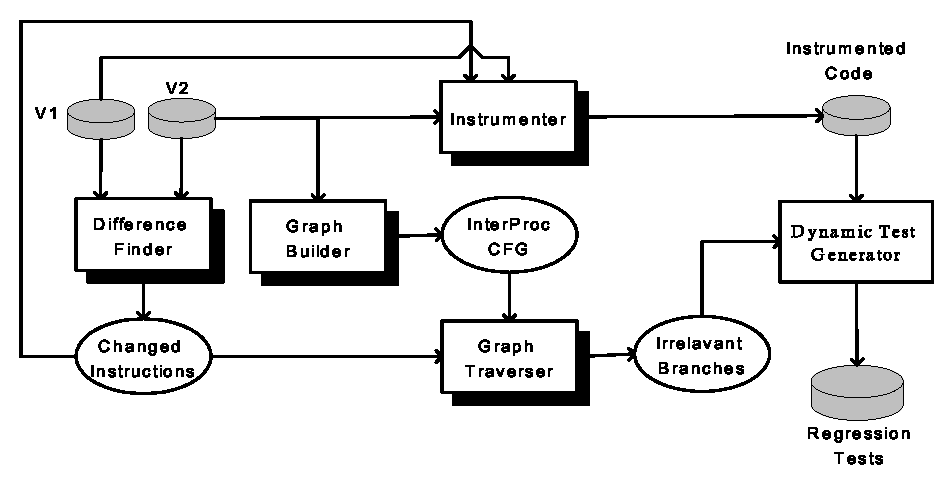
\includegraphics[width=8cm, keepaspectratio]{Figures/appr}
        \vspace{-0.35 in}
    \caption{Overview of \CodeIn{eXpress}}
    \label{fig:approach}
    \vspace{-0.15 in}
\end{figure}
}
\subsection{Difference Finder}
The \CodeIn{Difference Finder} component takes the two versions $v1$ and $v2$ as input and analyzes the two versions to find pairs $<M_{i1}, M_{i2}>$ of corresponding methods in $v1$ and $v2$, where $M_{i1}$ is a method in $v1$ and $M_{i2}$ is a method in $v2$. A method $M$ is defined as a triple $<FQN, Sig, I>$, where $FQN$ is the fully qualified name\footnote{\scriptsize{The fully qualified name of a method $m$ is a combination of the method's name, the name of the class $c$ declaring $m$, and the name of the namespace containing $c$.}} of the method, $Sig$ is the signature\footnote{\scriptsize{Signature of a method $m$ is the combination of parameter types of $m$ and the return type of $m$.}} of the method, and $I$ is the list of assembly instructions in the method body. Two methods $<M_{i1}, M_{i2}>$ form a  corresponding pair if the two methods $M_{i1}$ and $M_{i2}$ have the same $FQN$ and $Sig$. Currently our approach considers as different methods the methods that have undergone \CodeIn{Rename Method} or \CodeIn{Change Method Signature} refactoring. A refactoring detection tool~\cite{Dig'06:ECOOP} can be used to find such corresponding methods. For each pair $<M_{i1}, M_{i2}>$ of corresponding methods, the \CodeIn{Difference Finder} finds a set of  differences $\Delta_i$ between the list of instructions $I_{M_{i1}}$ and $I_{M_{i2}}$ in the body of Methods $M_{i1}$ and $M_{i2}$, respectively. $\Delta_i$ is a set of instructions such that each instruction $\iota$ in $\Delta_i$ is an instruction in $I_{M_{i2}}$ (or in $I_{M_{i1}}$ for a deleted instruction), and $\iota$ is added, modified, or deleted from list $I_{M_{i1}}$ to form $I_{M_{i2}}$.

In the rest of its components, \CodeIn{eXpress} analyzes Version $v2$ of the program while using the differences obtained from the \CodeIn{Difference Finder} component to efficiently generate regression tests. Note that Version $v1$ can also be used instead of $v2$ in path exploration.

\subsection{Graph Builder}
   
The \CodeIn{Graph Builder} component makes an inter-procedural control flow graph (CFG) of the program version $v_2$. The \CodeIn{Graph Builder} component starts the construction of the inter-procedural CFG from the Parametrized Unit Test (PUT) $\tau$ provided as input. The inter-procedural CFG is used by the \CodeIn{Graph Traverser} component to find branches (in the graph) via which the execution cannot reach any vertex containing a changed instruction in the graph.
\algsetup{indent=2em}
\newcommand{\factorial}{\ensuremath{\mbox{\sc Factorial}}}
%\vspace{- 0.25 in}
\begin{algorithm}[h!]
\begin{tiny}
\caption{$InterProceduralCFG(\tau)$}\label{alg:factorial}
\begin{algorithmic}[1]
\REQUIRE A test method $\tau$.
\ENSURE The inter-procedural Control Flow Graph (CFG) of the program under test.

\medskip

\STATE $Graph$ $g \leftarrow GenerateIntraProceduralCFG$($\tau$)
\FORALL {Vertex $v \in g.Vertices$}
\IF{v.Instruction = MethodInvocation}
 \STATE $c \leftarrow getMethod(v.Instruction)$
 \IF {$c \in MethodCallStack$}
 \STATE $goto$ Line 2 To avoid loops
 \ENDIF
 
 
 \IF{$c \in ReachableToChangedRegion$}
  \STATE $g \leftarrow GraphUnion(ChangedMethod, g, v)$ 
  \STATE $goto$ Line 2
 \ENDIF 
 
 \IF{$c \in Visited$}
  \STATE $goto$ Line 2
 \ENDIF 
 
 \IF{$c \in ChangedMethods$}
	 \STATE $ChangedMethod \leftarrow c $
	 \FORALL {Method $m \in MethodCallStack$}
		 \STATE $ReachableToChangedRegion.Add(m)$	
 	 \ENDFOR
 \ENDIF
 
 
 		
 \STATE $MethodCallStack.Add(c)$
 \STATE $cg \leftarrow InterProceduralCFG(c)$ 
 \STATE $MethodCallStack.Remove(c)$
 \STATE $Visited.Add(c)$
 
 \STATE $g \leftarrow GraphUnion(cg, g, v)$
 \ENDIF
\ENDFOR
\RETURN $g$
%\caption{Pseudocode of Construction of Inter-Procedural Control Flow Graph}
\label{alg:ICFG}
\end{algorithmic}
\end{tiny}
\end{algorithm}
Since a moderate-size program can contain millions of method calls (including those in its dependent libraries), often the construction of inter-procedural graph is not scalable to real-world programs. Hence, we build a minimal inter-procedural CFG for which our purpose of finding branches not reachable to some changed region in the program can be served. The pseudo code for building the inter-procedural CFG is shown in Algorithm~\ref{alg:factorial}. Initially, the algorithm \CodeIn{InterProceduralCFG} is invoked with the argument as the PUT \CodeIn{$\tau$}. An intra-procedural CFG $g$ is constructed for the method $\tau$. 
For each method invocation vertex\footnote{\scriptsize{A \CodeIn{method invocation vertex} is a vertex representing a call instruction.}} (invoking Method $c$) in $g$, the algorithm \CodeIn{InterProceduralCFG} is invoked recursively with the invoked method $c$ as the argument (Line 22 of Algorithm~\ref{alg:factorial}), while adding $c$ to the call stack (Line 21). After the control returns from the recursive call, the method $c$ is removed from the call stack (Line 23) and added to the set of visited methods (Line 24). The inter-procedural graph \CodeIn{cg} (with $c$ as an entry method) resulting from the recursive call at Line 22 is merged with the graph $g$ (Line 25).
\Comment{
To avoid loops in method invocations, the method \CodeIn{InterProceduralCFG} is not invoked recursively with $c$ as argument if $c$ is already in the call stack (Lines 5-6). In addition, thee method \CodeIn{InterProceduralCFG} is not invoked recursively with $c$ as argument if $c$ is already visited (Lines 23). 
If a changed method\footnote{\scriptsize{A changed method $M_i$ is a method for which the set $\Delta_i \neq \phi $.}} is encountered, the methods in the call stack are added to the set \CodeIn{ReachableToChangedRegion} (Lines 17-19). Finally, if a method $c$ in \CodeIn{ReachableToChangedRegion} is encountered, the method \CodeIn{InterProceduralCFG} is not invoked recursively with $c$ as argument, while merging CFG of some changed method with $g$. Since our aim of building the intra-procedural graph is to find branches in the graph that are not reachable to any changed instruction, the previous step helps in achieving the aim while reducing the cost of building the inter-procedural CFG. In addition, the size of the inter-procedural graph is also reduced which results in reduction in the cost of finding branches not reachable to the changed instructions.
}
The algorithm \CodeIn{InterProceduralCFG} is not invoked recursively with $c$ as argument in the following situations:
%\begin{itemize}
\\ \textbf{$c$ is in call stack.} If $c$ is already in the call stack, \CodeIn{InterProcedural CFG} is not recursively invoked with $c$ as argument (Lines 5-6). This technique ensures that our approach is not stuck in a loop in method invocations. For example, if method A invokes method B and method B invokes A. Then the construction of inter-procedural graph stops after A is encountered the second time.
\\ \textbf{ $c$ is already visited.} If $c$ is already visited, \CodeIn{InterProcedural CFG} is not recursively invoked with $c$ as argument (Lines 23). This technique ensures that we do not have to build the same subgraph again.
\\ \textbf{ $c$ is in \CodeIn{ReachableToChangedRegion}.} The set \CodeIn{ReachableToChanged Region} is populated whenever a changed method\footnote{\scriptsize{A changed method $M_i$ is a method for which the set $\Delta_i \neq \phi $.}} is encountered. In particular, if a changed method is encountered, the methods currently in the call stack are added to the set  \CodeIn{ReachableToChanged Region} (Lines 17-19). If $c$ is in \CodeIn{ReachableToChangedRegion}, \CodeIn{InterProceduralCFG} is not recursively invoked with $c$ as argument, while merging CFG of some changed method with $g$ (Line 8-11).
%\end{itemize}
Since our aim of building the intra-procedural CFG is to find irrelevant branches, those in the graph via which the execution cannot reach any changed instruction, the preceding three techniques help in achieving the aim while reducing the cost of building the inter-procedural CFG. In addition, the size of the inter-procedural CFG is reduced resulting in reduction in the cost of finding irrelevant branches.

\subsection{Graph Traverser}
The \CodeIn{Graph Traverser} component takes as input the inter-procedural CFG $g$ constructed by the \CodeIn{Graph Builder} component and a set $V$ of changed vertices in the CFG $g$. \CodeIn{Graph Traverser} traverses the graph to find a set of branches $B$ via which the execution cannot reach any of the branch in $V$. A branch $b$ in CFG $g$ is an edge $e = <v_i, v_j>: e \in g$ , where $v_i$ is a vertex in $g$ with a degree of more that one. The vertex $v$ is referred to as a branching node. The pseudo code for finding the set of branches $B$ is shown in Algorithm~\ref{alg:irrelavantBranches}.

\algsetup{indent=2em}
\newcommand{\UnrechableBranches}{\ensuremath{\mbox{\sc FindUnreachableBranches}}}
\begin{algorithm}[h!]
\begin{tiny}
\caption{$FindUnreachableBranches(g, V)$}\label{alg:irrelavantBranches}
\begin{algorithmic}[1]
\REQUIRE A Graph $g$ and a set $V$ of vertices in Graph $g$.
\ENSURE A set of branches $B$ in Graph $g$ that do not have a path to any vertex $v \in V$.

\medskip

\STATE $Reachable \leftarrow Reachable \cup V$
\FORALL {Vertex $v \in g.Vertices$ such that $v.degree > 1 $}
  
  \IF {$Reachable.Contains(v)$}
  	\STATE goto Line 2
  \ENDIF
  
	\STATE $\rho \leftarrow FindPathUsingDFS(v, V, Reachable)$
	
	\IF {$\rho$ is empty}
	  \FORALL {Vertex $n \in v.OutVertices$} 
			\STATE $B \leftarrow B \cup <v,n>$
		\ENDFOR
   	\STATE goto Line 2
	\ENDIF
		
	\FORALL {Vertex $pv \in \rho$ such that $v.degree > 1 $}
		\STATE $Reachable \leftarrow Reachable \cup pv$
	\ENDFOR
	
	\WHILE {$v.OutVertices \neq \phi$} 
	    \STATE $R \leftarrow R \cup <v, v_j>: v_j \in \rho$
			\STATE $g \leftarrow g.RemoveEdge(v, v_j)$
			\STATE $\rho \leftarrow FindPathUsingDFS(v, V, Reachable)$
			\IF{$\rho$ is empty}
					\FORALL {Vertex $o \in v.OutVertices$} 
						\STATE $B \leftarrow B \cup <v,o>$
					\ENDFOR
					\STATE $g \leftarrow g.AddEdges(R$)
					\STATE goto Line 2
			\ENDIF	
	\ENDWHILE
	\STATE $g \leftarrow g.AddEdges(R)$	
\ENDFOR
\RETURN $B$
\label{alg:ICFG}
\end{algorithmic}
\end{tiny}
\end{algorithm}


For each Vertex $v$ in $g$ such that $degree(v) > 1$, the \CodeIn{Graph Traverser} performs a depth first search (DFS) from Vertex $v$ (Line 6) to finds a path between $v$ and some vertex $c \in V$.
\Comment{ (the pseudo code of DFS is shown in Algorithm~\ref{alg:DFS}).
\algsetup{indent=2em}
\newcommand{\DFS}{\ensuremath{\mbox{\sc DFS}}}
\begin{algorithm}[h!]
\begin{tiny}
\caption{$FindPathUsingDFS(g, v, R)$}\label{alg:DFS}
\begin{algorithmic}[1]
\REQUIRE A Graph $g$, a vertex $v$ in the graph $g$, a set of vertices $R$.
\ENSURE A path $\rho$ in Graph $g$ from Vertex $v$ to Vertex $c \in V$.

\medskip

\STATE $v.Visited \leftarrow true$;
\STATE $\rho$.Append(v)
\IF {$v \in R$}
	\RETURN $\rho$
\ENDIF	
\FORALL {Vertex $n$ in v.OutVertices}
	\IF{$n.Visited \neq true$}
		\STATE goto Line 6 
	\ENDIF
	\STATE $\rho$.Append(n);
	\IF {$n \in R$}
		\RETURN $\rho$
	\ENDIF
	\STATE $\varrho \leftarrow FindPathUsingDFS(g, n, R)$
	\IF {$\varrho$ is not empty}
	  \RETURN $\varrho$
	\ENDIF
	\STATE $\rho.Remove(n)$

\ENDFOR
\STATE $\rho$.Remove(v)
\RETURN $\phi$
\label{alg:ICFG}
\end{algorithmic}
\end{tiny}
\end{algorithm}
}
If no path is found, all branches $b_i = <v, v_i>$ are added to the set $B$ (Lines 7-10) since none of these branches have a path to any of the vertices in $V$. If a path $\rho$ is discovered (Lines 16-27 in Algorithm~\ref{alg:irrelavantBranches}) by the DFS, there may still be a branch $b_i = <v, v_i>$ that is not reachable to any vertex $c \in V$. To find such branch, we remove the edge $e_j=<v, v_j>: e_j \in \rho$ from the graph and perform DFS again starting from $v$. We repeat the preceding steps until we either find no path $\rho$ or all the edges from $v$ are removed from the graph. If no path is found, the branches from v containing the remaining vertices are added to the set $B$ (Lines 21-23). 

To make the traversal efficient, whenever a path $\rho$ is found, all the vertices $r: degree(r)>1$ are added to the set of $Reachable$. This technique can help in making the future runs of DFS efficient. Whenever a vertex in the set $Reachable$ is encountered, the DFS is stopped; returning the current path.
 
\subsection{Instrumenter}
\Comment{
The \CodeIn{Instrumenter} component transforms the two versions of the program code such that the transformed program code is amenable to regression testing. In particular, our approach instruments both versions of the program under test. The instrumentation allows us to compare the internal behavior of running the same generated test on the two versions. 
}

The \CodeIn{Instrumenter} component uses Sets $\Delta_i$ (differences between method $M_{i1}$ and $M_{i2}$) produced by the \CodeIn{Difference Finder}. For each changed method pair $<M_{i1}, M_{i2}>$ for which $\Delta_i \neq \phi$, the \CodeIn{Instrumenter} component finds a region $\delta_i$ containing all the changed instructions in the program. $\delta_i$ is a minimal list of continuous instructions such that all the changed instructions in the method $M_i$ are in the region $\delta_i$. Hence, there can be a maximum of one changed region in one method. At the end of each changed region $\delta_i$, the \CodeIn{Instrumenter} component inserts instructions to save the program state. In particular, the \CodeIn{Instrumenter} inserts the corresponding instructions for \CodeIn{PexStore} statements for each variable (and field) defined in the changed region.
The \CodeIn{PexStore} statement for a variable $x$ results in an assertion statement \CodeIn{PexAssert.IsTrue( "uniqueName", x == currentX)} in the generated test, where \CodeIn{currentX} is the value of $x$ at Line 12 in the new version of the example program in Figure~\ref{fig:example}.
The \CodeIn{Dynamic Test Generator} component generates tests for the new version $v2$.
Once a test is generated that executes a changed region, 
the test is executed on Version $v1$ 
to compare program states after the execution of the changed region
with the ones captured in the execution of Version $v2$.



\subsection{Dynamic Test Generator}

The \CodeIn{Dynamic Test Generator} component performs Dynamic Symbolic Execution (DSE)~\cite{Clarke:symbolic, king:symex, dart, cute, exe} to 
generate regression tests for the two given versions of a program. DSE iteratively generates test inputs to cover various feasible paths in the program under test (the new version in our approach). In particular, DSE flips some branching node discovered in previous executions to generate a test input for covering a new path. The node to be flipped is decided by a search strategy such as depth-first search. 
The exploration is quite expensive since there are an exponential 
number of paths with respect to the number of branches in a program.
 However, the execution of many branches often cannot help in detecting behavioral differences. 
 In other words, covering these branches does not help in satisfying any of the condition E or I in the PIE model described in Section~\ref{sec:intro}. 
 Therefore, we do not flip such branching nodes in our new search strategy for generating test inputs that detect 
 behavioral differences between the two given versions of a program. Recall that, we refer to such branches as irrelevant branches. These branches are found using the  \CodeIn{Graph Traversal} component.
 We next describe the two categories of paths that our approach avoids exploring, and then describe their corresponding branches.
 
 \subsubsection{Paths being Pruned}
 Our approach avoids exploring the following categories of paths:
 \Comment{
%\begin{itemize}
\\ \textbf{Rationale E: Paths not leading to any changed region.} Paths that cannot reach any changed region (denoted as $\delta$) need not be 
explored. For example, consider the \CodeIn{testMe} program in Figure~\ref{fig:example}.
 The changed statement is at Line 11 ($\delta$). While searching for a path 
 to cover $\delta$, we do not need explore paths containing the \CodeIn{true} branch of the condition at Line 8. 
\\ \textbf{Rationale I: Paths not causing any state infection.} Suppose that we cover $\delta$ at Line 11 
in Figure~\ref{fig:example} using inputs \CodeIn{x=90} and the array \CodeIn{y} of length 20 where each element of \CodeIn{y} has a value 15. The execution takes a path $P$ 
executing the loop 20 times, assigning the variable \CodeIn{x} to 110 and eventually 
covering $\delta$ at Line 11 . However, the program state after the execution of $\delta$ is not infected since 
after the first execution of $\delta$, the value of \CodeIn{x} is 3 in both versions. We need not explore the subpaths after the execution of a changed region that does not cause any state infection if these subpaths do not lead to any other changed region.
\Comment{
\item \textbf{Rationale P: Paths not propagating state infection to any observable output.} Suppose $\delta$ is executed, the program state is infected after the execution of $\delta$, but the infection does not propagate to an observable output. Let $\chi$ be the statement at which infection propagation stops. We need not explore the subpaths after the execution of $\chi$ if these subpaths do not lead to any other changed region.	 
}
%\end{itemize}
\subsubsection{Branching Nodes being Pruned}
In DSE, path exploration is realized by flipping branching nodes. We next describe two categories of branching nodes that we avoid flipping corresponding to the preceding two categories of paths that we intend to avoid exploring.
}%\begin{itemize}
\\ \textbf{Category E. }Let $V={v_1,v_2,..,v_n}$ be the set of all vertices in CFG $g$ such that $ v_i \in g$ and $v_i.degree >1$ . Let $E_i = {e_{i1}, e_{i2},...,e_{in}}$ be the set of outgoing edges (branches) from $v_i$. Let $C$ be the set of changed vertices in $g$, $\rho(v_i, C, e_{ij})$ denotes a path (if exists) between a vertex $v_i$ to any vertex in set $C$ that takes the branch $e_{ij}$ of Vertex $v_i$.
For all vertices $v_i \in V$, our approach avoids from exploring all the branches $e_{ij}\in E_i : \rho(v_i, C, e_{ij}) = \phi$ (such branches are found using \CodeIn{Graph Traverser} component). In other words, if an instance of branching node $v_i$ is in the discovered dynamic execution tree\footnote{\scriptsize{A dynamic execution tree is the tree formed from the paths executed in the previous executions. Multiple instances $c_{i1}, c_{i2}, ..., c_{in}$ of a node $c_i$ in CFG can be present in a dynamic execution tree due to loops in a program.}}, such that the branch $e_{ij}$ is not explored yet, our approach does not flip $v_i$ to make program execution take branch $e_{ij}$.
As an effect, our approach helps reduce the number of paths to be explored by avoiding the paths $P \in g : e_{ij} \in P$.
\\
\textbf{Category I. }
Let $C \in g$ be the set of nodes in all the changed regions.
Let some $c_i \in C$ be executed i.e  at lease one instance $c_{ij}$ of $c_i$ is present in the dynamic execution tree $T$. Consider that the program state is not infected after the execution of changed region containing $c_i$. Our approach prunes all the branching nodes $B \in T$, such that for all $b_i \in B: \rho(c_{ij}, b_i) \neq \phi, b_i \notin C $, where $\rho(c_i, b_i)$ is the path between the vertices $c_i$ and $b_i$ (if exists) in $T$. As an effect of pruning $B$, our approach does not explore the subpaths after the execution of a changed region that does not cause any state infection.
\Comment{
\\ \textbf{Category E.} This category contains all the branching nodes whose the other unexplored branch cannot lead to any changed region. These branches are obtained from the \CodeIn{Graph Traversal} component, which traverses the inter-procedural CFG constructed by the \CodeIn{Graph Builder} component.
\\
\textbf{Category I.} If a changed region is executed but the program state is not infected after the execution of the changed region, all the branching nodes after the changed region $\delta$ in the current execution path are included in this category. These branches are obtained by inspecting the path $P$ followed in the previous DSE run. Let $P = <b_1, b_2,.., b_c...b_n>$, where $b_i$ are the branching nodes in the Path $P$, while $b_c$ is the last instance of branching node containing $\delta$. We do not flip the branching nodes from $b_c$ to $b_n$ in $P$ if the program state is not infected.
%\Comment{
\item \textbf{Category P.} Consider that a changed region is executed and the program state is infected after the execution of the changed region; However, the infection is not propagated to any observable output. Let $\chi$ be the last location in the execution path such that the program state is infected before the execution of $\chi$ but not infected after its execution. $\chi$ can be determined by comparing the value spectra~\cite{xie05:spectra} obtained by executing the test on both versions of the program. This category contains all the branching nodes after the execution of $\chi$. These branches are obtained by inspecting the path $P$ followed in the previous DSE run. Let $P = <b_1, b_2,.., b_\chi...b_n>$, where $b_i$ are the branching nodes in the Path $P$, while $b_\chi$ is the last instance of the branching node containing $\chi$. We do not flip the branching nodes from $b_\chi$ to $b_n$ in $P$ until the program state.	 
}
%\end{itemize}
\Comment{
\subsubsection{Branching Nodes being Prioritized}
In addition to avoiding flipping the preceding categories of branching nodes, we prioritize branching nodes to be flipped after each run of DSE based on the distance of the branching node to a changed region in the CFG. The distance $d(n1, n2)$ between any two nodes $n1$ and $n2$  in a CFG $g$ is the number of nodes with degree > 1 between $n1$ and $n2$ in the shortest path between $n1$ and $n2$. Hence, the distance between a node $b$ and $\delta$ is the number of nodes with degree more than one between $b$ and the node representing the first instruction in $\delta$   The intuition behind this prioritization is that lesser the distance between the branching node and $\delta$, it is likely to be easier to generate inputs to cause the execution of the changed region $\delta$. This kind of branch prioritization is also used by Burnim and Sen~\cite{burnim}.
}
\subsection{Incremental Test Generation}
\label{sec:incremental}
A regression test suite achieving high code coverage may be available along with the original version of  a program. This test suite may be manually written or generated by an automated test generation tool for the original version. However, the existing test suite might not be able to cover all the changed parts of the new version of the program. Our approach can reuse the existing test suite so that changed parts of the program can be executed efficiently due to which test generation is likely to find behavior differences earlier in path exploration. Our approach executes the existing test suite to build an execution
tree for the tests in the test suite. Our approach then starts the program
exploration using the dynamic execution tree instead of starting from an empty
tree. Our approach of seeding test inputs can help efficiently cover the changed parts of the program with two major reasons:
\\ \textbf{Discovery of hard to discover branching nodes.} By seeding the existing test suite to Pex, our approach executes the test suite to build an execution tree of the program (discovered by executing the existing test suite). Some of the branches in the discovered execution tree may take a large number of DSE runs (without seeding any tests) to get discovered. Flipping some of these discovered branching nodes nearer in CFG to the changed parts of the
program has more likelihood of covering the changed regions of the program~\cite{burnim}. Although, currently, our approach does not specifically prioritize the flipping of the branches near to the changed parts, our approach can help these branches to get discovered, which might take large number of DSE runs as shown in the example in Section~\ref{sec:example}.
\\ \textbf{Priority of DSE to cover not covered parts of the program.} DSE techniques employ branch prioritization so that a high coverage can be achieved faster due to which DSE techniques choose a branch from the execution tree (discovered thus far) that have a high likelihood of covering new program parts. By seeding the existing test suite to program exploration, the DSE techniques do not waste time on covering the parts of the program already covered by the existing test suite. Instead, the DSE techniques give priority to branching nodes that can cover new parts of the program, which include the changed parts. Hence, the changed parts are likely to be covered earlier in path exploration.
 
 \Comment{
Pex then focuses on flipping the unexplored branches to effectively cover the changed parts of the program.
Even seeding a single test that covers portions of the program neared in CFG to the changed parts  can help the program exploration in effectively covering the changed parts of the program because various branches are discovered in the execution tree that are, which otherwise might take a number of runs in .
Hence choosing the number of tests in the test suite to seed is an optimization problem. In section, ??? we conduct experiments by increasing the number of seeds. by seeding (1)one closest pest to the changes (2) seding tests that achieve a high block coverage (3) seeding tests that achieve a higher path coverage, to assess whether seeding more tests helps the path exploration.
We found out that tests achieving a high block coverage performs the best.
}


 
 